% Szglab4
% ===========================================================================
%
\chapter{Prototípus koncepciója}

\thispagestyle{fancy}

\setcounter{section}{-1}
\section{Módosítások a specifikációban}

\subsection{Ragacs kopása}
\textbf{A ragacs eltűnik a pályáról, miután négy robot ráugrott (elkopik).}\newline
A Sticky osztályban létrehozunk egy változót, ami nyilvántartja, hogy hányan ugrottak rá. Ezt a változót az osztály visit(Robot element) metódusa fogja menedzselni.

\subsection{Olaj felszáradása}
\textbf{Egy meghatározott idő letelte után az olajfolt eltűnik a pályáról (felszárad).}\newline
Az Oil osztályban létrehozunk egy változót, ami nyilvántartja a hátralévő idejét. A hátralévő időt úgy menedzseli, hogy az osztály implementálja a HeartBeatListener interfészt és az onTick(long deltaTime) metódusában levonja az eltelt időt.

\subsection{Robotok ütközése}
\textbf{A robotok képesek ütközni, ha azonos helyre érkeznek ugrásuk végén. Ilyenkor a gyorsabb robot összetöri (megsemmisíti) a lassabbat, és kettejük átlagsebességével halad tovább (vektorátlag!).}\newline
A Field onEnter(Agent agent) metódusában, ha a Field-en éppen van egy másik Agent is, akkor meghívjuk a Fielden az éppen rajtalévő Agent collide(Agent agent) metódusát. A collide-ban a vesztesre meghívjuk az agent.accept(new KillExecute) metódust.

\clearpage

\subsection{Osztálydiagram módosítások}
\begin{figure}[h]
	\begin{center}
		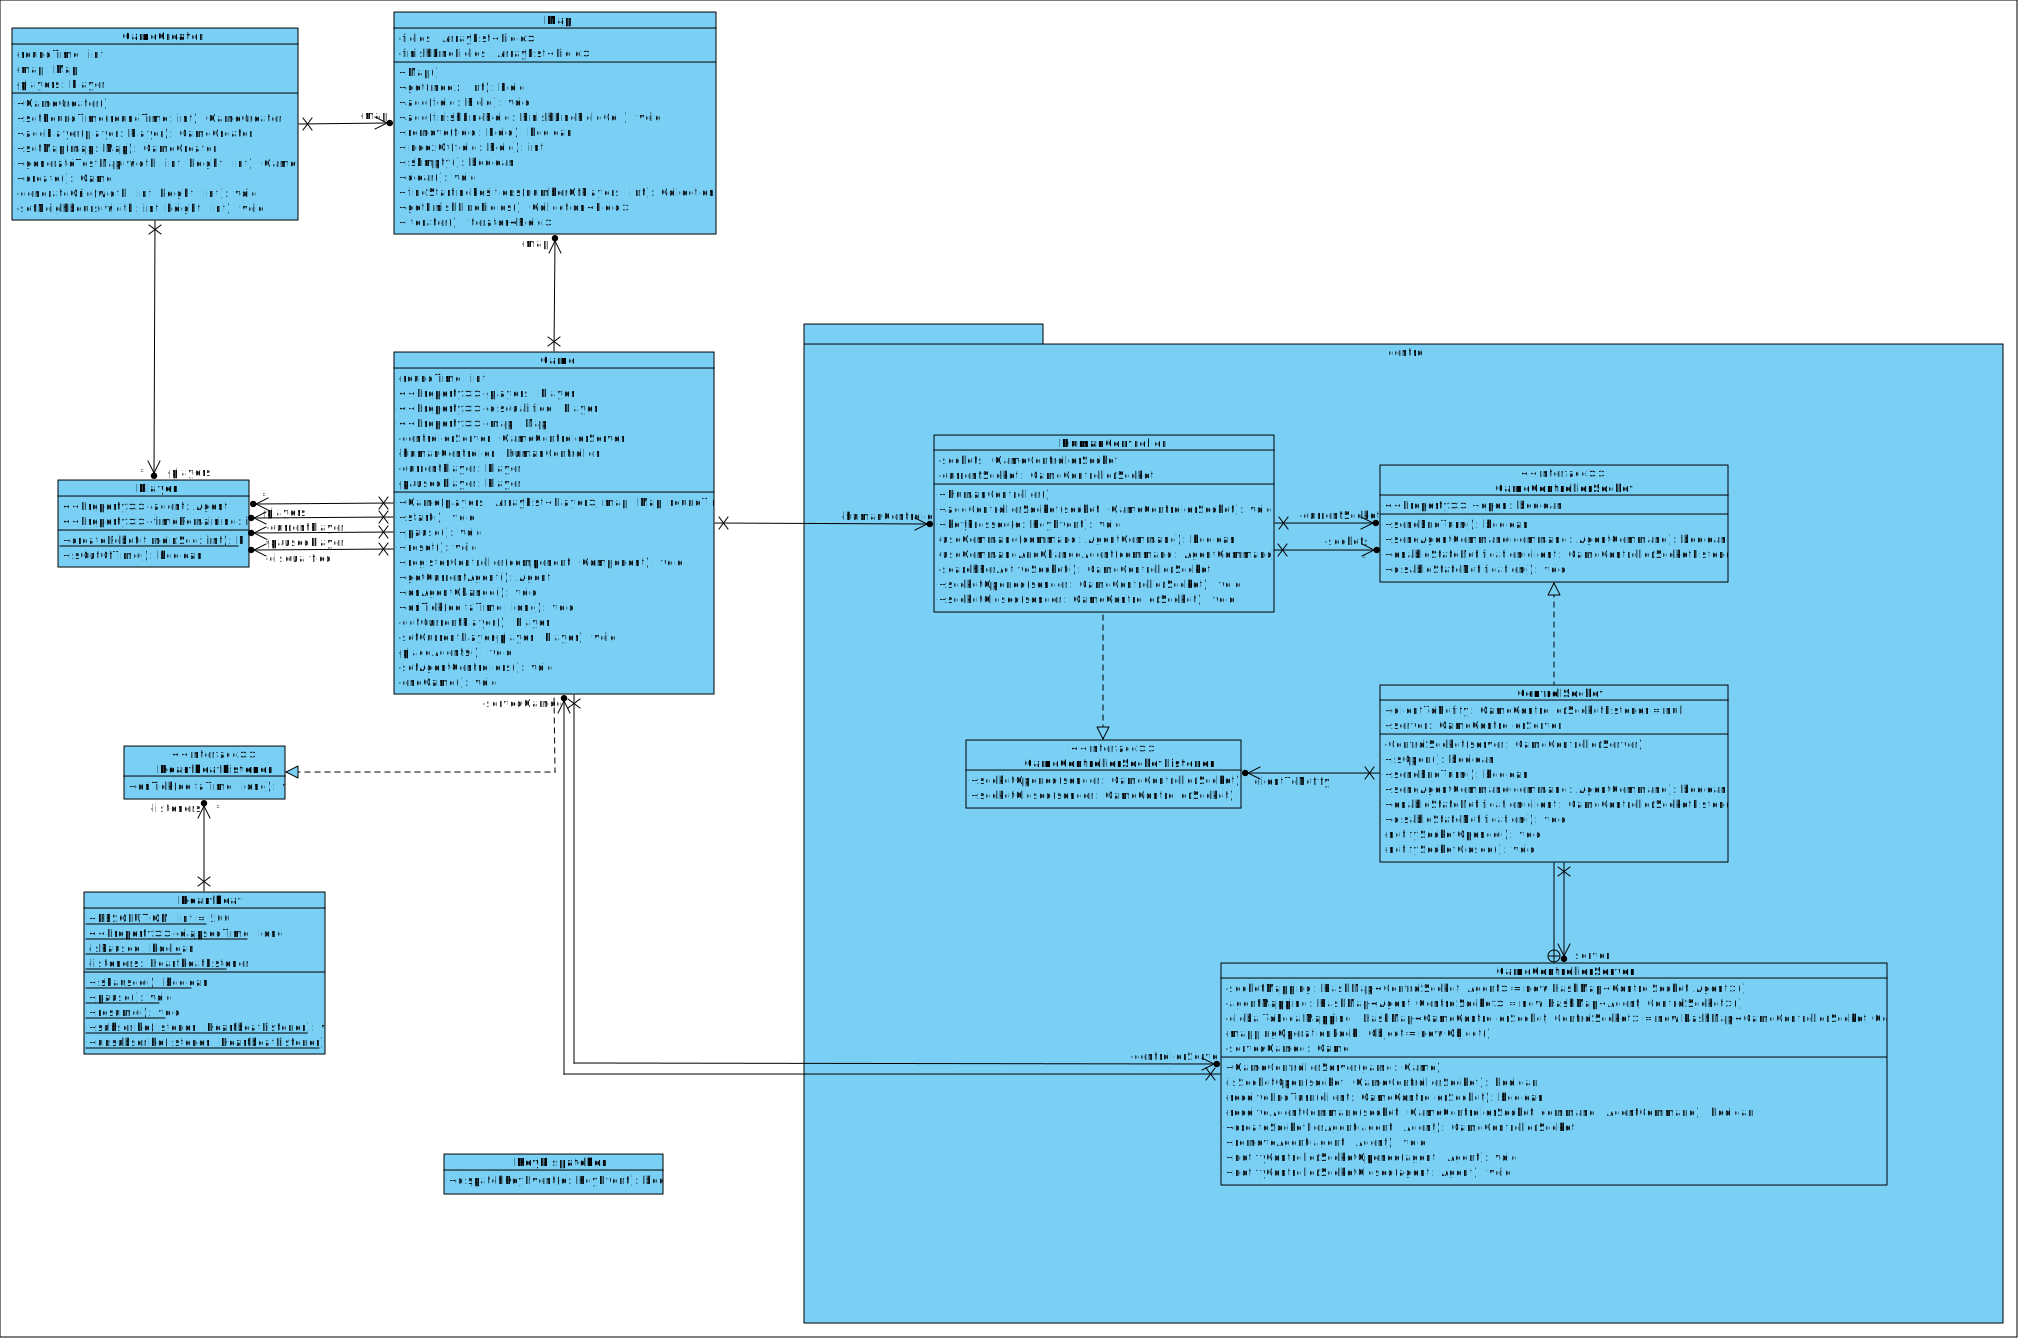
\includegraphics[width=\linewidth]{chapters/chapter07/gamepackage.pdf}
		\caption{Game package osztálydiagram}
		\label{Game package osztálydiagram}
	\end{center}
\end{figure}

\clearpage


\subsection{Szekvenciadiagram módosítások}
\begin{figure}[h]
	\begin{center}
		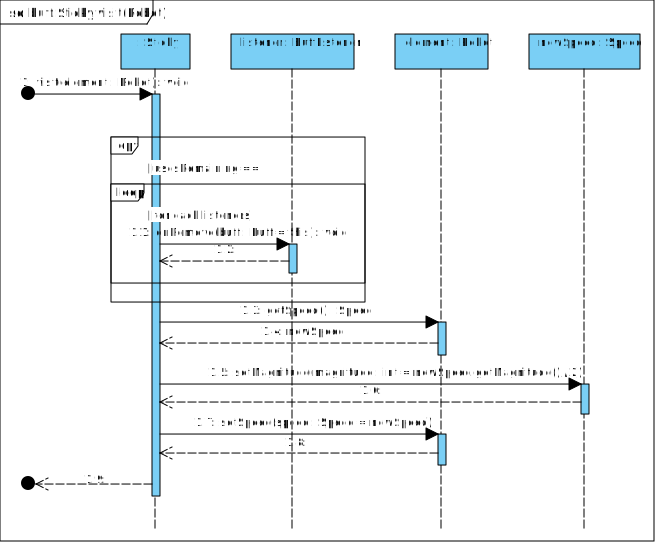
\includegraphics[width=\linewidth]{chapters/chapter07/ragacskopas.pdf}
		\caption{Ragacs kopása}
		\label{Ragacs kopása}
	\end{center}
\end{figure}

\clearpage

\begin{figure}[h]
	\begin{center}
		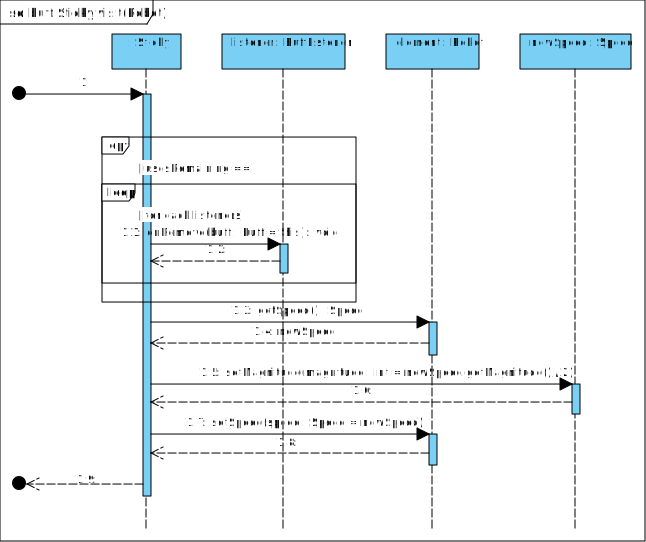
\includegraphics[width=\linewidth]{chapters/chapter07/olajszaradas.pdf}
		\caption{Olaj felszáradása}
		\label{Olaj felszáradása}
	\end{center}
\end{figure}

\clearpage

\begin{figure}[h]
	\begin{center}
		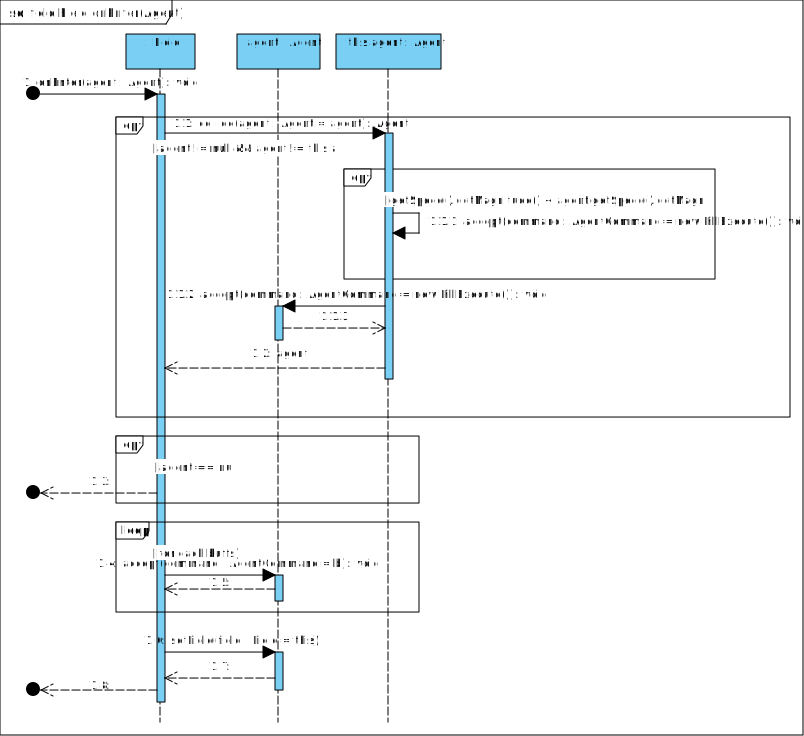
\includegraphics[width=\linewidth]{chapters/chapter07/utkozes.pdf}
		\caption{Robotok ütközése}
		\label{Robotok ütközése}
	\end{center}
\end{figure}

\clearpage


\section{Prototípus interface-definíciója}

\subsection{Az interfész általános leírása}
Az interfész a szabványos bemenetről tud fogadni parancsokat, a kimenetet pedig a szabványos kimenet jelenti. Ennek köszönhetően a használat
leegyszerűsödik, mivel a ki/bemenetek átirányításával lehetőség adódik ki/bemeneti fileokat megadni, melyek lehetőséget adnak a helyes működés
ellenőrzésére, amennyiben összehasonlításra kerülnek egy referenciakimenettel (mely az elvárt működést írja le.). Egy teszteset a prototípusnak
adható parancsok szekvenciájából, kimenet pedig az ezekre adott válaszokból áll. A tesztet sikeresnek mondhatjuk, ha a referenciakimenettel 
megegyező eredményt produkál. \\
A -rng kapcsolóval lehetőség adódik a randomizálható értékek generálására. Ezen kapcsoló hiányában a program tökéletesen determinisztikusan működik,
ez a funkció csak a tesztelői input rövidítésére szolgál. Viszont nem használható automata ellenőrzés esetén.\\
A -log kapcsoló lehetőséget ad a logok szintjének állítására például all/test/debug. \\

\subsection{Bemeneti nyelv}
A bemeneti nyelv az alábbi általános szintaxist használja: 

\lstset{escapeinside=`', xleftmargin=10pt, frame=single, basicstyle=\ttfamily\footnotesize, language=sh}
\begin{lstlisting}
parancs(arg1=ertek1, arg2=ertek2, arg3=ertek3)
\end{lstlisting}

\noindent A parancs végét a sor vége jelzi. Bármely parancs tetszőleges számú szóközzel tagolható, de a kis- és nagybetűket megkülönböztetik: az előző példával így egyenértékű például:

\lstset{escapeinside=`', xleftmargin=10pt, frame=single, basicstyle=\ttfamily\footnotesize, language=sh}
\begin{lstlisting}
parancs (arg1 = ertek1,arg2 = ertek2,arg3 = ertek3)
\end{lstlisting}

\noindent De külöböző tőle:

\lstset{escapeinside=`', xleftmargin=10pt, frame=single, basicstyle=\ttfamily\footnotesize, language=sh}
\begin{lstlisting}
PARANCS(arg1=ertek1, arg2=ertek2, arg3=ertek3)
\end{lstlisting}

\begin{itemize}

    \item jatek(szam=n, ido=m, palya=nev.map)
	\begin{itemize}
	    \item Leírás: Új játék kezdésére használt parancs.
	    \item Opciók:
            \begin{itemize}
                \item szam: a játékosok száma (2-4)
                \item ido: az egy játékosra jutó köridő
                \item palya: a betöltendő pálya neve
            \end{itemize}
	\end{itemize}
    
    \item betolt(nev=allas.sav)
    \begin{itemize}
        \item Leírás: Egy mentett játékállás betöltése
        \item Opciók: 
            \begin{itemize}
                \item nev: a mentett játékallás neve
            \end{itemize}
    \end{itemize}
    
    \item ment(nev=allas.sav)
    \begin{itemize}
         \item Leírás: Az aktuális játékállás elmentése
         \item Opciók: 
             \begin{itemize}
                 \item nev: a mentett játékallás neve
             \end{itemize}
    \end{itemize}

    \item ugrik()
    \begin{itemize}
        \item Leírás: Az aktuálisan soron lévő ágenset utasítja ugrásra
        \item Opciók: 
    \end{itemize}
    
    \item irvalt(irany=IRANY)
    \begin{itemize}
        \item Leírás: Az aktuálisan soron lévő ágens sebességének irányát változtatja meg
        \item Opciók: 
            \begin{itemize}
                \item irany: az új irány (lehetséges értékek: FEL, LE, BAL, JOBB)
            \end{itemize}
    \end{itemize}
    
    \item sebvalt(delta=n)
    \begin{itemize}
        \item Leírás: Az aktuálisan soron lévő ágens sebességének nagyságát változtatja
        \item Opciók: 
            \begin{itemize}
                \item delta: A változtatás nagysága (a program felülírhatja a felhasználó döntését, amennyiben az kívül esik az általa várt tartományon) 
            \end{itemize}
    \end{itemize}

    \item olajlerak()
    \begin{itemize}
        \item Leírás: Az aktuálisan soron lévő ágenset utasítja egy olajfolt lehelyezésére
        \item Opciók: 
    \end{itemize}

    \item ragacslerak()
    \begin{itemize}
        \item Leírás: Az aktuálisan soron lévő ágenset utasítja egy ragacsfolt lehelyezésére
        \item Opciók: 
    \end{itemize}
    
    \item vacuumlerak(field=fieldid)
    \begin{itemize}
    	\item Leírás: Lerak egy adott field-re egy kisrobotot.
       	\item Opciók: 
            \begin{itemize}
                  	\item field: Az adott field fieldid-ja
            \end{itemize}	
    \end{itemize}
    
    \item robotlerak(field=fieldid)
    \begin{itemize}
    	\item Leírás: Lerak egy adott field-re egy robotot
    	\item Opciók: 
    	\begin{itemize}
    		\item field: Az adott field fieldid-ja
    	\end{itemize}	
    \end{itemize}      
    
    \item olajleptet(ido=s)
    \begin{itemize}
    	\item Leírás: Az olaj hátralévő idejéből levesz s időt.
    	\item Opciók: 
    	\begin{itemize}
    		\item ido: A levonásra váró idő szekundumban
    	\end{itemize}	
    \end{itemize}
    
    \item olajlerak(field=fieldid)
    \begin{itemize}
       	\item Leírás: Lerak egy adott field-re egy olajat
       	\item Opciók: 
       	\begin{itemize}
       		\item field: Az adott field fieldid-ja
       	\end{itemize}	
    \end{itemize}
    
    \item ragacslerak(field=fieldid)
    \begin{itemize}
    	\item Leírás: Lerak egy adott field-re egy ragacsot
    	\item Opciók: 
    	\begin{itemize}
    		\item field: Az adott field fieldid-ja
    	\end{itemize}	
    \end{itemize}    
    
    \item vacuumtakarit()
    \begin{itemize}
    	\item Leírás: Elkezd takarítani a cellán, amin épp van. Ha nincs a cellán olaj, akkor nem takarít.
    	\item Opciók: 
    \end{itemize}    

    

\end{itemize}

\noindent A pályaképet a Java beépített szerializációs formátumában tároljuk, erről részletes leírás az alábbi linken olvasható:\\
\url{http://docs.oracle.com/javase/7/docs/platform/serialization/spec/serialTOC.html}

\subsection{Kimeneti nyelv}

A gömbölyű zárójellel ellátott részletek csak megjegyzések, a kimenetben nem szerepelnek. \newline

\begin{itemize}
	\item Irányváltoztatás
	\begin{itemize}
		\item Kimenet <sikeres \{0\} | sikertelen \{1\}>
		\begin{itemize}
				\item \{0\} Robot: <robotid> Új irány: <újirány>
				\item \{1\} (Sikertelen irányváltoztatás) Robot: <robotid>
		\end{itemize}
	\end{itemize}
	
	\item Sebesség változtatás
	\begin{itemize}
		\item Kimenet <sikeres \{0\} | sikertelen \{1\}>
		\begin{itemize}
			\item \{0\} Robot: <robotid> Új sebesség: <újsebesség>
			\item \{1\} (Sikertelen sebesség változtatás) Robot: <robotid>
		\end{itemize}
	\end{itemize}
	
	\item Ugrás
	\begin{itemize}
		\item Kimenet <sikeres \{0\} | sikertelen \{1\}>
		\begin{itemize}
			\item \{0\} Robotid: <robotid> Előző cella: <fieldid> Új cella: <fieldid>
			\item \{1\} (Sikertelen ugrás) Robot: <robotid>
		\end{itemize}
	\end{itemize}
	
	\item Olaj lerakása cellára
	\begin{itemize}
		\item Kimenet <sikeres \{0\} | sikertelen \{1\}>
		\begin{itemize}
			\item \{0\} Robot: <robotid>  Érintett cella: <fieldid>
			\item \{1\} (Sikertelen olaj lerakás) Robot: <robotid>
		\end{itemize}
	\end{itemize}
	
	\item Ragacs lerakása cellára
	\begin{itemize}
		\item Kimenet <sikeres \{0\} | sikertelen \{1\}>
		\begin{itemize}
			\item \{0\} Robot: <robotid>. Érintett cella: <fieldid>
			\item \{1\} (Sikertelen ragacs lerakás) Robot: <robotid>
		\end{itemize}
	\end{itemize}	
	
	\item Új játék kezdése
	\begin{itemize}
		\item Kimenet <sikeres \{0\} | sikertelen \{1\}>
		\begin{itemize}
			\item \{0\} Generált pálya: <Map> Generált robotok: <Robot>
			\item \{1\} (Sikertelen mentés.)
		\end{itemize}
	\end{itemize}
	
	
	\item Játék elmentése
	\begin{itemize}
		\item Kimenet <sikeres \{0\} | sikertelen \{1\}>
		\begin{itemize}
			\item \{0\} Sikeres mentés megadott elérési útvonalra. 
			\item \{1\} (Sikertelen mentés.)
		\end{itemize}
	\end{itemize}

	\item Játék betöltése
	\begin{itemize}
		\item Kimenet <sikeres \{0\} | sikertelen \{1\}>
		\begin{itemize}
			\item \{0\} Betöltött pálya: <Map> Betöltött robotok <Robot> 
			\item \{1\} (Sikertelen betöltés.)
		\end{itemize}
	\end{itemize}
	
	\item Vacuum lerakása adott cellára
	\begin{itemize}
		\item Kimenet <sikeres \{0\} | sikertelen \{1\}>
		\begin{itemize}
			\item \{0\} Vacuum: <vacuumid> on Field: <fieldid> Célolaj on {<fieldid> | null}
			\item \{1\} (Sikertelen lerakás.)
		\end{itemize}
	\end{itemize}	
	
	\item Robot lerakása adott cellára
	\begin{itemize}
		\item Kimenet <sikeres \{0\} | sikertelen \{1\}>
		\begin{itemize}
			\item \{0\} Robot: <robotid> on Field: <fieldid> 
			\item \{1\} (Sikertelen lerakás.)
		\end{itemize}
	\end{itemize}	
	
	\item Olaj léptetése adott idővel
	\begin{itemize}
		\item Kimenet <sikeres \{0\} | sikertelen \{1\}>
		\begin{itemize}
			\item \{0\} Hátralévő idő: <ido> 
			\item \{1\} (Sikertelen leptetes.)
		\end{itemize}
	\end{itemize}	
	
	\item Olaj lerakása adott cellára
	\begin{itemize}
		\item Kimenet <sikeres \{0\} | sikertelen \{1\}>
		\begin{itemize}
			\item \{0\} Field: <fieldid> 
			\item \{1\} (Sikertelen lerakás.)
		\end{itemize}
	\end{itemize}	
	
	\item Ragacs lerakása adott cellára
	\begin{itemize}
		\item Kimenet <sikeres \{0\} | sikertelen \{1\}>
		\begin{itemize}
			\item \{0\} Field: <fieldid> 
			\item \{1\} (Sikertelen lerakás.)
		\end{itemize}
	\end{itemize}		
	
	\item Vacuum utasítása takarításra
	\begin{itemize}
		\item Kimenet <sikeres \{0\} | sikertelen \{1\}>
		\begin{itemize}
			\item \{0\} Hatralevo kor: <n>
			\item \{1\} (Sikertelen takarítás.) notarget
		\end{itemize}
	\end{itemize}
	
\end{itemize}


\section{Összes részletes use-case}
%\comment{A use-case-eknek a részletezettsége feleljen meg a kezelői felületnek, azaz a felület elemeire kell hivatkozniuk.}
Alábbi táblázat minden use-case-hez külön-külön.

\usecase%
{Új játék indítása}%
{Elindíthatunk egy új játékot}%
{Játékos, Játék}%
{A játékosok számának megadása után a Játékos kezdeményezheti a játéknak az elindítását}

\usecase%
{Játékparaméterek megadása}%
{Új játék paramétereinek megadása}%
{Játék}%
{Játékosok megadhatják, hogy hányan vannak, milyen időkorláttal kívánnak játszani}

\usecase%
{Játék megnyerése}%
{Játék végső helyzete alapján győztes eldöntése}%
{Játékos, Játék}%
{Ha minden Játékosnak lejár akkor a megtett út alapján eldől, hogy ki a győztes}

\usecase%
{Játék elvesztése}%
{Játék végső helyzete alapján vesztesek eldöntése}%
{Játékos, Játék}%
{Ha minden Játékosnak lejár akkor a megtett út alapján eldől, hogy kik a vesztesek}

\usecase%
{Játék elmentése}
{A játék jelenlegi állásának fájl(ok)ba mentése}
{Játékos, Játék}
{A Játékos megadja az elérési utat és a Játék elmenti a játékot}

\usecase%
{Játék betöltése}
{A játék fájlból való betöltése}
{Játékos, Játék}
{A Játékos megadja az elérési utat és a Játék betölti a játékot}

\usecase%
{Logolás}
{A játékos meghatározza, hogy logoljon a program}
{Játékos, Játék}
{A Játékos beállítja a logolás mértékét a -log kapcsolóval}

\usecase%
{Randomizálás}
{A játékos meghatározza, hogy véletlenszerű értékekkel működjön a program}
{Játékos, Játék}
{A Játékos az -rng kapcsolóval tudja ezt állítani}


\section{Tesztelési terv}
%\comment{A tesztelési tervben definiálni kell, hogy a be- és kimeneti fájlok egybevetésével miként végezhető el a program tesztelése. Meg kell adni teszt forgatókönyveket. Az egyes teszteket elég informálisan, szabad szövegként leírni. Teszt-esetenként egy-öt mondatban. Minden teszthez meg kell adni, hogy mi a célja, a proto mely funkcionalitását, osztályait stb. teszteli. Az alábbi táblázat minden teszt-esethez külön-külön elkészítendő.}

Tesztelést egy összetett parancssorozat végrehajtásával fogjuk elvégezni. Egy általunk megtervezett paranccsorozatot készítünk a bemeneti nyelven melyet az "Az interfész általános leírása" részben leírt módon átadunk a programnak. Tartalmazni fogja a felsorolt tesztesetek minden elemét oly módon hogy azokkal vizsgálható legyen a helyes működésnek a menete az esetlegesen játék szabályait nem követő utasítások ellenében is. Valamint előre elkészül egy kimeneti nyelven megírt helyes végrehajtásra utaló kimenet melyet a program össze tud vetni az általa generált kimenettel. A felhasználó számára pedig mutatja az egyező és eltérő sorokat is. 

\teszteset{Új játék indítása}%
{Elindítunk egy új játékmenetet}%
{Meggyőződés arról, hogy a program képes a játékkörnyezetet kialakítani vagy betölteni a megadott paraméterek alapján}

\teszteset{Új játék paramétereinek megadása}%
{Beállíthatjuk milyen pályán kívánnak a felhasználók játszani és hányan.}%
{Megvizsgálni, hogy tényleg megfelelően tárolódtak-e el a megadott paraméterek mely az új játékmenet kialakításához kell}

\teszteset{Pálya betöltése}%
{Eltárolt pályának a betöltése a játékhoz}%
{Meggyőzödhetünk általa, hogy az elmentett pála betöltését a program el tudja-e megfelelően végezni}

\teszteset{Új táték indítása}%
{Elindítunk egy új játékmenetet}%
{Meggyőződés arról, hogy a program képes a játékkörnyezetet kialakítani vagy betölteni a megadott paraméterek alapján}

\teszteset{Robot sebességének változtatása}%
{Egy robot sebességét, mely az ugrásának a vektoriális elmozdulását adja, tudjuk így meghatározni}%
{A sebesség tényleges megválozásának kimutatása és meghatározása}

\teszteset{Robot utasítása olaj lehelyezésére}%
{Egy robotot utasíthatunk arra, hogy a pályán hagyjon ott egy olajfoltot, mellyel más játékosokat hátráltatni tud}%
{A lehelyezés elvégézésének a biztosítása}

\teszteset{Robot utasítása ragacs lehelyezésére}%
{Egy robotot utasíthatunk arra, hogy a pályán hagyjon ott egy ragacsfoltot, mellyel más játékosokat hátráltatni tud}%
{A lehelyezés elvégézésének a biztosítása}

\teszteset{Robot utasítása másik robotra való ráugrásra}%
{Egy robot ha egy olyan mezőre ugrik melyen már van Robot, akkor a megadott feltételek alapján a gyengébb haladhat tovább}%
{Vizsgálandó, hogy tényleg a megfelelő Robot esik-e ki ebben az állapotban}

\teszteset{Pályáról lelépő robotot elakaszt}%
{Amennyiben egy robot lelép a pálya határain kívülre, akkor ezzel kiesik a játékból, nem tud többet mozogni}%
{Az elakasztás megtörténtének megvizsgálása}

\teszteset{Robot utasítása ugrásra}%
{Egy robotot utasíthatunk arra, hogy ugorjon, ezzel mozgást végezve a pályán, mely szügséges ahhoz, hogy elérhesse a játék célját}%
{Az ugrás végrehajtásának megtörténtének és más robotokkal ez során végzett interakciók biztosítása}

\teszteset{Olajos mező sebességváltoztatást nem enged}%
{Egy robottal olajos mezőre lépve a robot azt az akadályoztatást szenvedi el, hogy nem változtathatja meg sebességét}%
{Ellenőrizni, hogy egy ilyen folttal rendelkező mezőn egy, a robotnak adott sebességváltoztatás utasítás nem kerül érvényre}

\teszteset{Ragacsos mező sebességet megfelez}%
{Egy robotal ragacsos mezőre lépve az robot azt az akadályoztatást szenvedi el, hogy sebessége megfeleződik}%
{Ellenőrizni, hogy egy ilyen folttal rendelkező mezőn egy a robotnak a sebessége valóban megfeleződik}

\teszteset{Takarító robot működésének ellenőrzése}%
{A pályán időnként megjelenő takarító robotok melyek a foltokat takarítják le a pályáról}%
{Cél hogy ellenőrizzük, hogy ezek a robotok valóban találnak-e koszos mezőt és azt letakarítják-e}

\section{Tesztelést támogató segéd- és fordítóprogramok specifikálása}
A csapat a tesztelést támogató progamot egy egyszerű különbségellenőrzőnek képzeli el, mely képes a kimenetet egy referenciafilelal összehasonlítva megmondani,
hogy az output melyik sorában van eltérés a várt kimenettől. Ennek segítségével lehetőség nyílik a hiba felderítésére és javítására. Bemenetei a program által adott
teszteset outputja és a referenciafile. Kimenete az eltérések. 

